\section{Experimental Setup}

\subsection*{Circuit components}
    \begin{enumerate}
        \item A PNP transistor (CK100) 
        \item An NPN transistor (CL100)
        \item Resistors (4 nos.)
        \item D.C. power supply
        \item Multimeters (3 nos.)
        \item Connecting wires
        \item Breadboard
    \end{enumerate}

    \subsection*{Circuit Diagrams}
    \begin{figure}[H]
        \centering
        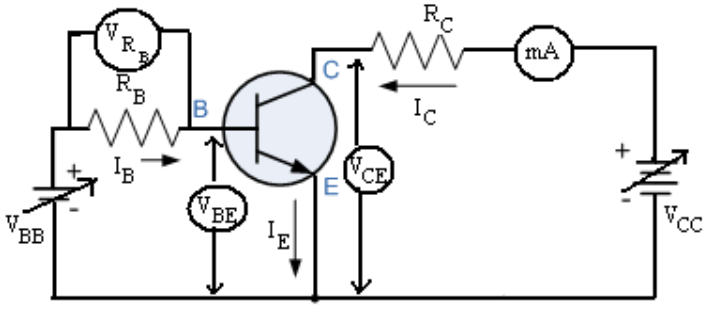
\includegraphics[width=.9\columnwidth]{images/ce.png}
        \caption{NPN transistor in CE configuration}
        \label{fig:1}
    \end{figure}

    \begin{figure}[H]
        \centering
        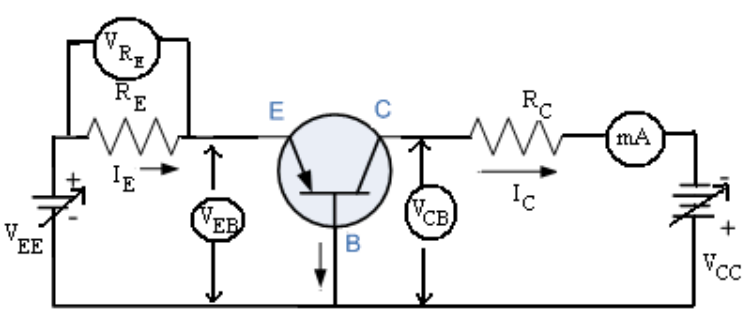
\includegraphics[width=.9\columnwidth]{images/cb.png}
        \caption{PNP transistor in CB configuration}
        \label{fig:2}
    \end{figure}

\section{Data Analysis}

\subsection{CE configuration}

\begin{itemize}
    \item Transistor code: CL100 (NPN)
    \item $R_B = 99\,k\Omega, R_C = 993\,\Omega$
\end{itemize}

    \subsubsection*{\textbf{Input Characterstics}} 

    \begin{figure}[H]
        \centering
        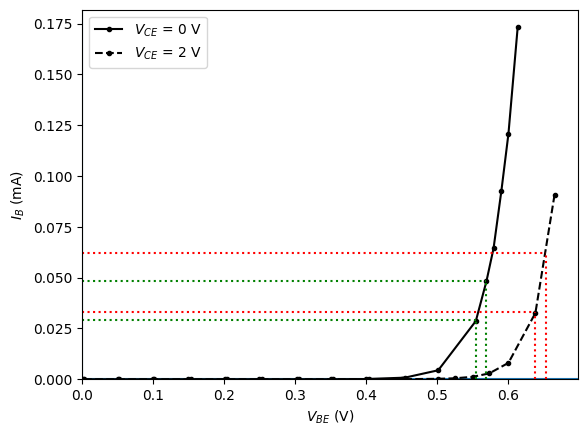
\includegraphics[width=1\columnwidth]{images/g1.png}
        \caption{Input characterstics of the NPN transistor in CE mode for different values of $V_{CE}$}
        \label{graph:1}
    \end{figure}

   

    From Eq. (5), input dynamic resistance can be calculated as the inverse of slope of the I-V curve in Fig. \ref{graph:1}. This comes out to be, 

    \begin{itemize}
        \item for $V_{CE}=0$ V, $r_i=769.23\,\Omega$ 
        \item for $V_{CE}=2$ V, $r_i=517.24\,\Omega$ 
    \end{itemize}

    \subsubsection*{\textbf{Output Characterstics}} 

    \begin{figure}[H]
        \centering
        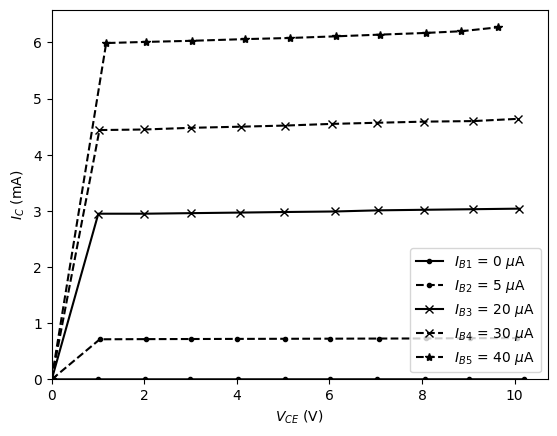
\includegraphics[width=1\columnwidth]{images/g2.png}
        \caption{Output characterstics of the NPN transistor in CE mode for different values of $I_{B}$}
        \label{graph:2}
    \end{figure}

  

    From Eq. (6), output dynamic resistance can be calculated as the inverse of slope of the I-V curve in the active region of the plot in Fig. \ref{graph:2}. This comes out to be, 

    \begin{itemize}
        \item for $I_B=0\,\mu$A, $r_o=8019.39\,k\Omega$ 
        \item for $I_B=5\,\mu$A, $r_o=399.89\,k\Omega$ 
        \item for $I_B=20\,\mu$A, $r_o=101.00\,k\Omega$ 
        \item for $I_B=30\,\mu$A, $r_o=50.47\,k\Omega$ 
        \item for $I_B=40\,\mu$A, $r_o=36.47\,k\Omega$ 
    \end{itemize}

    The high magnitudes of $r_o$ is due to the reverse biased state of the base-collector diode, in the active state.

    \subsubsection*{\textbf{Transfer Characterstics}} 

    \begin{figure}[H]
        \centering
        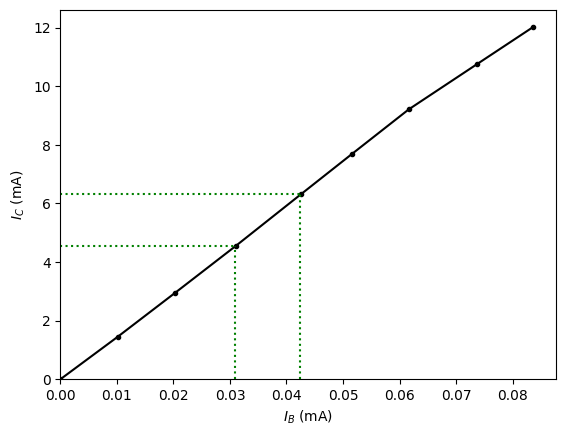
\includegraphics[width=1\columnwidth]{images/g3.png}
        \caption{Transfer characteristics of the NPN transistor in CE mode for a fixed $V_{CE}=1$ V}
        \label{graph:3}
    \end{figure}

    From Eq. (7), the current amplification factor can be calculated from as the slope of the $I_C$ vs $I_B$ curve in  Fig. \ref{graph:3}. This comes out to be $\beta_{ac}=154.78$. Since the plot is linear, the value of $\beta_{dc}$ (from Eq. (8)) can also said to be equal to $154.78$.

\subsection{CB configuration}

\begin{itemize}
    \item Transistor code: CK100 (PNP)
    \item $R_E = R_C = 151.1\,\Omega$
\end{itemize}

    \subsubsection*{\textbf{Input Characterstics}} 

    \begin{figure}[H]
        \centering
        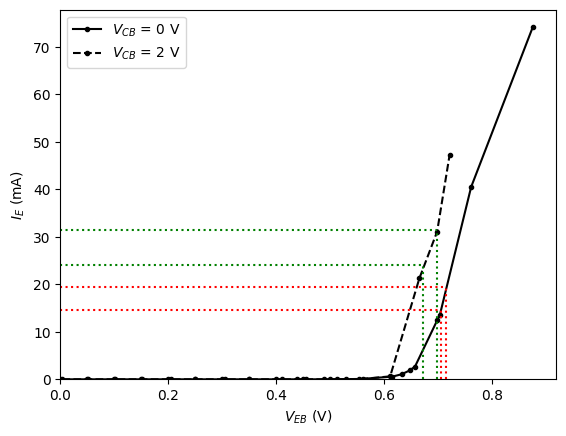
\includegraphics[width=1\columnwidth]{images/g4.png}
        \caption{Input characterstics of the PNP transistor in CB mode for different values of $V_{CB}$}
        \label{graph:4}
    \end{figure}


    From Eq. (1), input dynamic resistance can be calculated as the inverse of slope of the I-V curve in Fig. \ref{graph:4}. This comes out to be, 

    \begin{itemize}
        \item for $V_{CB}=0$ V, $r_i=3.51\,\Omega$ 
        \item for $V_{CB}=2$ V, $r_i=2.13\,\Omega$ 
    \end{itemize}

    \subsubsection*{\textbf{Output Characterstics}} 

    \begin{figure}[H]
        \centering
            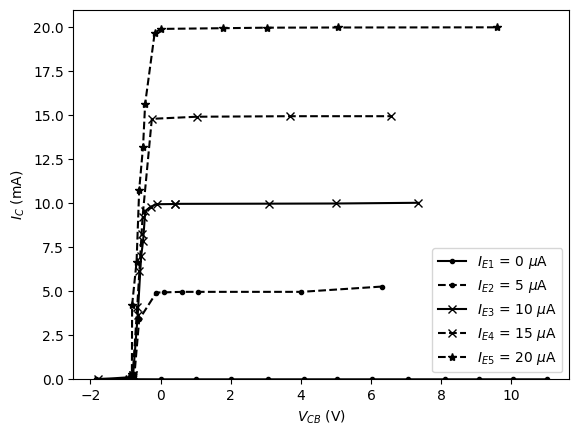
\includegraphics[width=\columnwidth]{images/g5.png}
           \caption{Output characterstics of the PNP transistor in CB mode for different values of $I_{E}$}
           \label{graph:5}
   \end{figure}

   

    From Eq. (2), output dynamic resistance can be calculated as the inverse of slope of the I-V curve in the active region of the plot in Fig. \ref{graph:5}. This comes out to be, 

    \begin{itemize}
        \item for $I_E=0\,\mu$A, $r_o=9700.00\,k\Omega$ 
        \item for $I_E=5\,\mu$A, $r_o=18.97\,k\Omega$ 
        \item for $I_E=10\,\mu$A, $r_o=192\,k\Omega$ 
        \item for $I_E=15\,\mu$A, $r_o=88.33\,k\Omega$ 
        \item for $I_E=20\,\mu$A, $r_o=202.70\,k\Omega$ 
    \end{itemize}

    \subsubsection*{\textbf{Transfer Characterstics}} 

    \begin{figure}[H]
        \centering
        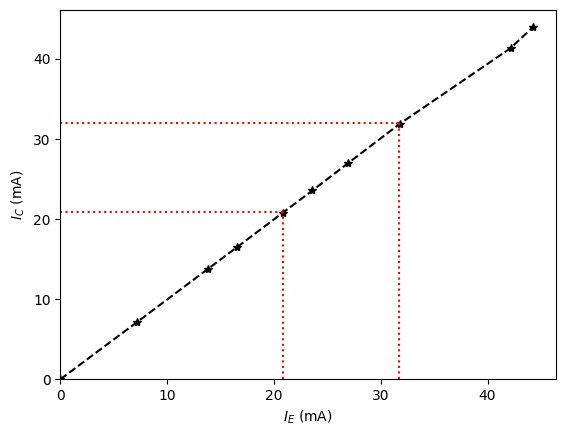
\includegraphics[width=1\columnwidth]{images/g6.png}
        \caption{Transfer characteristics of the PNP transistor in CB mode for a fixed $V_{CB}=1$ V}
        \label{graph:6}
    \end{figure}

    From Eq. (3), the current amplification factor can be calculated from as the slope of the $I_C$ vs $I_E$ curve in  Fig. \ref{graph:3}. This comes out to be $\alpha_{ac}=1.02$. Since the plot is linear, the value of $\alpha_{dc}$ (from Eq. (4)) can also said to be equal to $1.02$.

